\chapter{Samenvattende Schema's}
\section{Zoekmethodes}
\label{app:schemaSearch}
\begin{figure}[H]
\centering
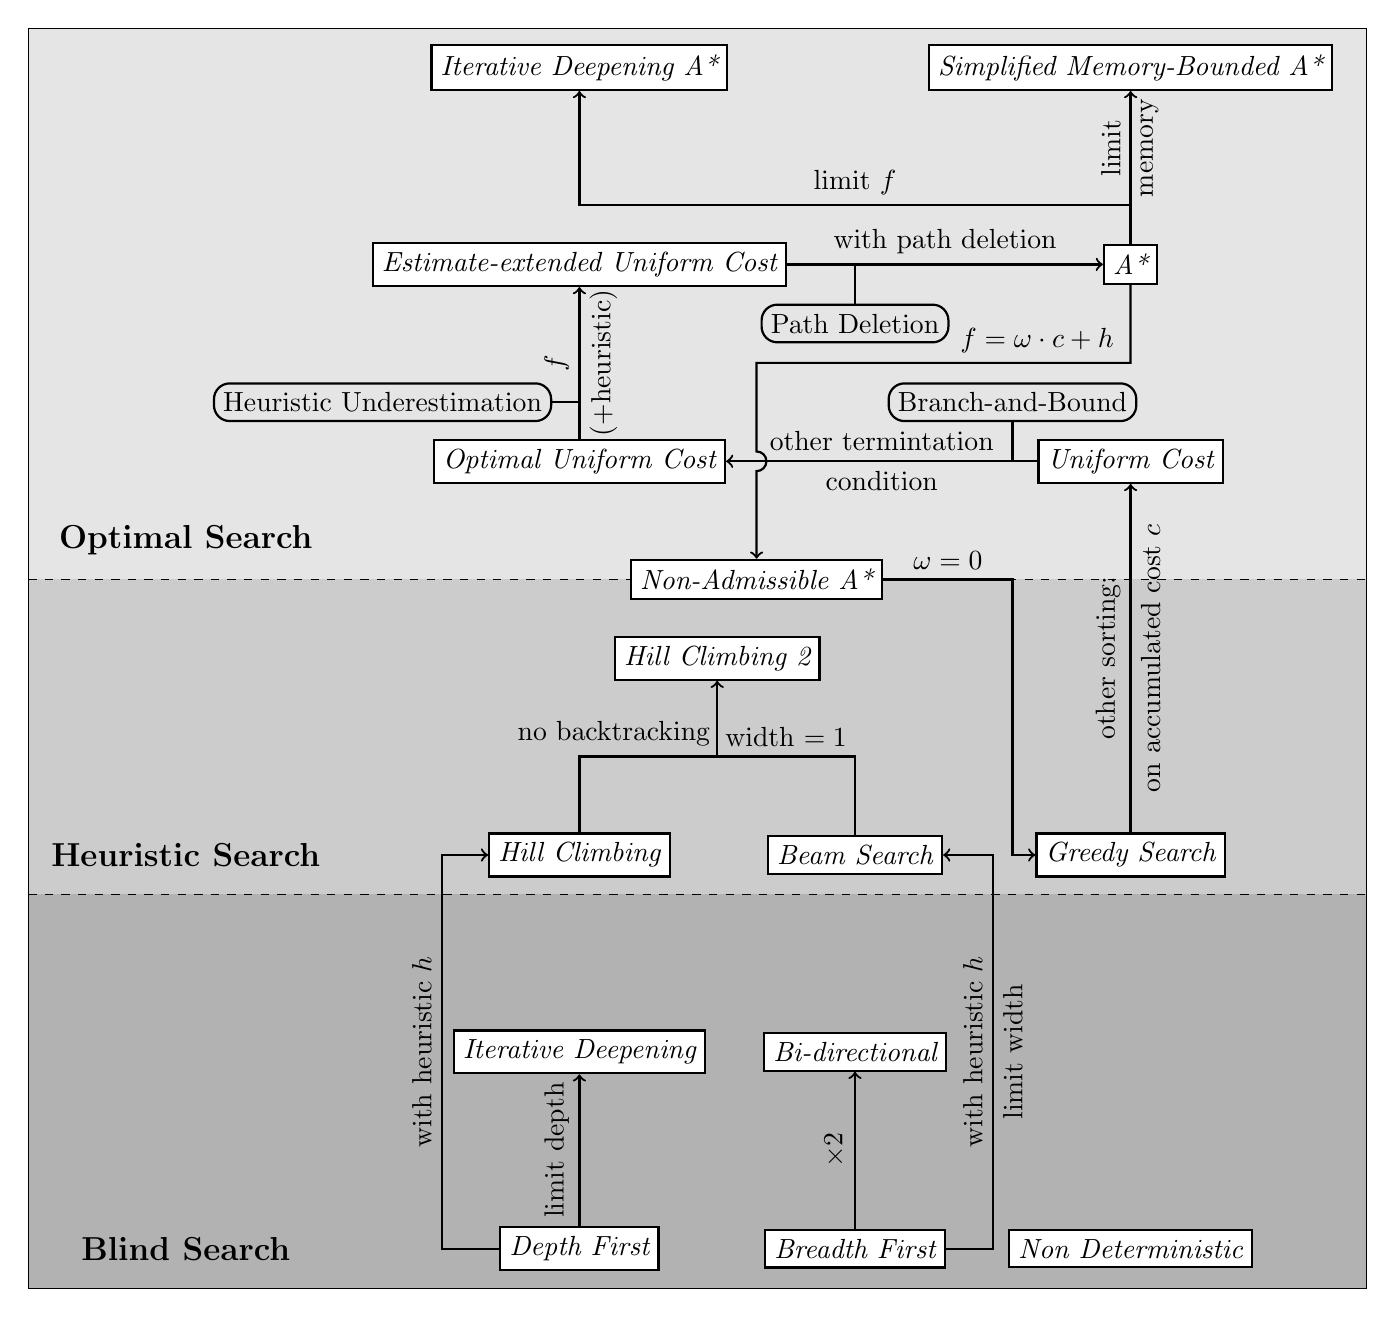
\begin{tikzpicture}[algor/.style={draw=black,thick,fill=white,font=\itshape},principle/.style={shape=rectangle,rounded corners=2mm,draw=black,thick,fill=black!10},hasinspired/.style={thick,->},hasinspirednoarrow/.style={thick},withprinciple/.style={thick,}]
\fill[black!30] (-2,-0.5) rectangle (15,4.5);
\fill[black!20] (-2,4.5) rectangle (15,8.5);
\fill[black!10] (-2,8.5) rectangle (15,15.5);
\draw (-2,-0.5) rectangle (15,15.5);
\draw[dashed] (-2,4.5) -- (15,4.5);
\draw[dashed] (-2,8.5) -- (15,8.5);
\draw[double] (0,0) node{\bf \large Blind Search};
\draw (0,5) node{\bf \large Heuristic Search};
\draw (0,9) node{\bf \large Optimal Search};
\node[algor] (df) at (5,0) {Depth First};
\node[algor] (bf) at (8.5,0) {Breadth First};
\node[algor] (nd) at (12,0) {Non Deterministic};
\node[algor] (id) at (5,2.5) {Iterative Deepening};
\node[algor] (bd) at (8.5,2.5) {Bi-directional};
\node[algor] (hc) at (5,5) {Hill Climbing};
\node[algor] (bs) at (8.5,5) {Beam Search};
\node[algor] (hc2) at (6.75,7.5) {Hill Climbing 2};
\node[algor] (gs) at (12,5) {Greedy Search};
\node[algor] (uc) at (12,10) {Uniform Cost};
\node[algor] (ouc) at (5,10) {Optimal Uniform Cost};
\node[algor] (euc) at (5,12.5) {Estimate-extended Uniform Cost};
\node[algor] (as) at (12,12.5) {A*};
\node[algor] (idas) at (5,15) {Iterative Deepening A*};
\node[algor] (smbas) at (12,15) {Simplified Memory-Bounded A*};
\node[algor] (naas) at (7.25,8.5) {Non-Admissible A*};
\node[principle] (bab) at (10.5,10.75) {Branch-and-Bound};
\node[principle] (hu) at (2.5,10.75) {Heuristic Underestimation};
\node[principle] (pd) at (8.5,11.75) {Path Deletion};
\draw[hasinspired] (df) to node[midway,above,rotate=90]{limit depth} (id);
\draw[hasinspired] (bf) to node[midway,above,rotate=90]{$\times2$} (bd);
\draw[hasinspired] (df) -- (3.25,0) to node[midway,above,rotate=90]{with heuristic $h$} (3.25,5) -- (hc);
\draw[hasinspired] (bf) -- (10.25,0) to node[midway,above,rotate=90]{with heuristic $h$} node[midway,below,rotate=90]{limit width} (10.25,5) -- (bs);
\draw[hasinspired] (hc)  -- (5,6.25) to node[near start,above]{no backtracking}  (6.75,6.25) -- (hc2);
\draw[hasinspirednoarrow] (bs) -- (8.5,6.25) to node[midway,above]{width $=1$} (6.75,6.25);
\draw[hasinspired] (gs) to node[midway,above,rotate=90]{other sorting:} node[midway,below,rotate=90]{on accumulated cost $c$} (uc);
\draw[hasinspired] (uc) to node[midway,above]{other termintation} node[midway,below]{condition} (ouc);
\draw[withprinciple] (bab) -- (10.5,10);
\draw[hasinspired] (ouc) to node[midway,above,rotate=90]{$f$} node[midway,below,rotate=90]{(+heuristic)} (euc);
\draw[withprinciple] (hu) -- (5,10.75);
\draw[hasinspired] (euc) to node[midway,above]{with path deletion} (as);
\draw[withprinciple] (pd) -- (8.5,12.5);
\draw[hasinspired] (as) -- (12,13.25) to node[midway,above]{limit $f$} (5,13.25) -- (idas);
\draw[hasinspired] (12,13.25) to node[midway,above,rotate=90]{limit} node[midway,below,rotate=90]{memory} (smbas);
\draw[hasinspired] (naas)  to node[midway,above]{$\omega=0$} (10.5,8.5) |- (gs.west);
\draw[hasinspired] (as) -- (12,11.25) to node[near start,above]{$f=\omega\cdot c+h$} (7.25,11.25) -- (7.25,10.125) arc (90:-90:.125) -- (naas);
\end{tikzpicture}
\caption{Samenvattend schema van Zoekmethodes}
\end{figure}
\section{Constraint Processing}
\begin{figure}[H]
\centering
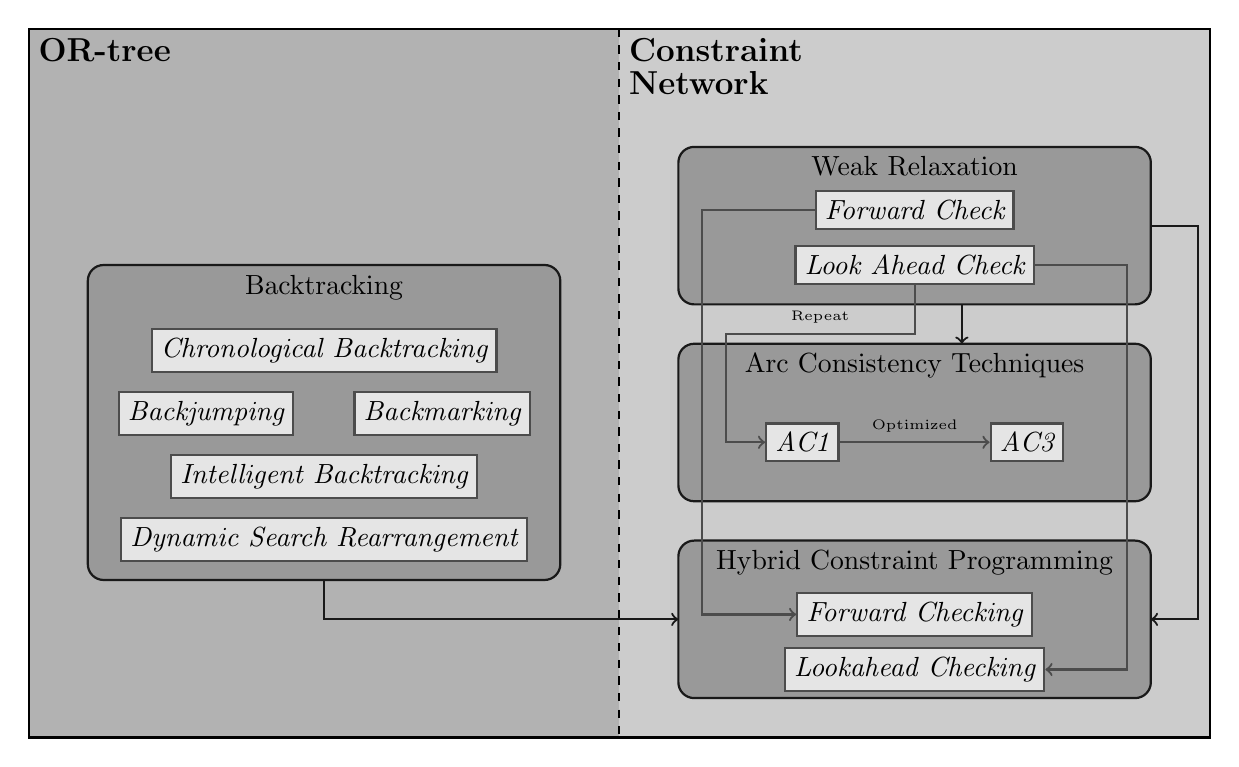
\begin{tikzpicture}[taal/.style={anchor=north west,text width=90pt},conceptgroup/.style={draw=black!90,fill=black!40, rounded corners=2mm, thick,minimum width=60mm,minimum height=20mm},hasinfluence/.style={black!90,thick,->},algor/.style={draw=black!70,thick,fill=black!10,font=\itshape},algorinfluence/.style={black!70,thick,->}]
\def\rectW{15};
\def\rectH{10};
\def\trapa{0};
\def\trapaCax{-0.25*\rectW+0.5*\trapa}
\def\trapaCay{-0.6*\rectH}
\def\trapaCaw{6}
\def\trapaCah{4}

\def\trapbCax{0.25*\rectW+0.5*\trapa}
\def\trapbCay{-0.35*\rectH}
\def\trapbCaw{6}
\def\trapbCah{2}
\def\trapbCbx{0.25*\rectW+0.5*\trapa}
\def\trapbCby{-0.6*\rectH}
\def\trapbCbw{6}
\def\trapbCbh{2}
\def\trapbCcx{0.25*\rectW+0.5*\trapa}
\def\trapbCcy{-0.85*\rectH}
\def\trapbCcw{6}
\def\trapbCch{2}

\fill[black!30] (-0.5*\rectW,-1) rectangle (\trapa,-\rectH);
\fill[black!20] (\trapa,-1) rectangle (0.5*\rectW,-\rectH);
\draw[thick] (-0.5*\rectW,-1) rectangle (0.5*\rectW,-\rectH);
\draw[thick,dashed] (\trapa,-1) -- (\trapa,-\rectH);

\node[taal] (trapaL) at (-0.5*\rectW,-1) {\bf \large OR-tree};
\draw[conceptgroup] (\trapaCax-0.5*\trapaCaw,\trapaCay-0.5*\trapaCah) rectangle (\trapaCax+0.5*\trapaCaw,\trapaCay+0.5*\trapaCah);
\node[anchor=north] (trapaG1) at (\trapaCax,\trapaCay+0.5*\trapaCah) {Backtracking};
\node[algor,anchor=north] (trapaG1A1) at (\trapaCax,\trapaCay+0.3*\trapaCah) {Chronological Backtracking};
\node[algor,anchor=north] (trapaG1A2) at (\trapaCax-0.25*\trapaCaw,\trapaCay+0.1*\trapaCah) {Backjumping};
\node[algor,anchor=north] (trapaG1A3) at (\trapaCax+0.25*\trapaCaw,\trapaCay+0.1*\trapaCah) {Backmarking};
\node[algor,anchor=north] (trapaG1A4) at (\trapaCax,\trapaCay-0.1*\trapaCah) {Intelligent Backtracking};
\node[algor,anchor=north] (trapaG1A5) at (\trapaCax,\trapaCay-0.3*\trapaCah) {Dynamic Search Rearrangement};

\node[taal] (trapbL) at (\trapa,-1) {\bf \large Constraint Network};
\draw[conceptgroup] (\trapbCax-0.5*\trapbCaw,\trapbCay-0.5*\trapbCah) rectangle (\trapbCax+0.5*\trapbCaw,\trapbCay+0.5*\trapbCah);
\node[anchor=north] (trapbG1) at (\trapbCax,\trapbCay+0.5*\trapbCah) {Weak Relaxation};
\node[algor] (trapbG1A1) at (\trapbCax,\trapbCay+0.1*\trapbCah) {Forward Check};
\node[algor] (trapbG1A2) at (\trapbCax,\trapbCay-0.25*\trapbCah) {Look Ahead Check};
\draw[conceptgroup] (\trapbCbx-0.5*\trapbCbw,\trapbCby-0.5*\trapbCbh) rectangle (\trapbCbx+0.5*\trapbCbw,\trapbCby+0.5*\trapbCbh);
\node[anchor=north] (trapbG2) at (\trapbCbx,\trapbCby+0.5*\trapbCbh) {Arc Consistency Techniques};
\node[algor,anchor=north] (trapbG2A1) at (\trapbCbx-0.2375*\trapbCbw,\trapbCby) {AC1};
\node[algor,anchor=north] (trapbG2A2) at (\trapbCbx+0.2375*\trapbCbw,\trapbCby) {AC3};
\draw[algorinfluence] (trapbG2A1) to node[above,midway,sloped,black]{\tiny Optimized} (trapbG2A2);
\draw[algorinfluence] (trapbG1A2.south) |-(\trapbCax,0.45*\trapbCay+0.55*\trapbCby) to node[above,midway,sloped,black]{\tiny Repeat} (\trapbCax-0.4*\trapbCaw,0.45*\trapbCay+0.55*\trapbCby) |- (trapbG2A1.west);
\draw[conceptgroup] (\trapbCcx-0.5*\trapbCcw,\trapbCcy-0.5*\trapbCch) rectangle (\trapbCcx+0.5*\trapbCcw,\trapbCcy+0.5*\trapbCch);
\node[anchor=north] (trapcG2) at (\trapbCcx,\trapbCcy+0.5*\trapbCch) {Hybrid Constraint Programming};
\node[algor,anchor=north] (trapbG3A1) at (\trapbCcx,\trapbCcy+0.175*\trapbCch) {Forward Checking};
\node[algor,anchor=north] (trapbG3A2) at (\trapbCcx,\trapbCcy-0.175*\trapbCch) {Lookahead Checking};
\draw[algorinfluence] (trapbG1A1.west) |- (\trapbCax-0.45*\trapbCaw,\trapbCay+0.1*\trapbCah) |- (trapbG3A1.west);
\draw[algorinfluence] (trapbG1A2.east) |- (\trapbCax+0.45*\trapbCaw,\trapbCay-0.25*\trapbCah) |- (trapbG3A2.east);
\draw[hasinfluence] (\trapbCax+0.5*\trapbCaw,\trapbCay) -- (\trapbCax+0.6*\trapbCaw,\trapbCay) |- (\trapbCcx+0.5*\trapbCaw,\trapbCcy);
\draw[hasinfluence] (\trapbCax+0.1*\trapbCaw,\trapbCay-0.5*\trapbCah) -- (\trapbCbx+0.1*\trapbCaw,\trapbCby+0.5*\trapbCbh);
\draw[hasinfluence] (\trapaCax,\trapaCay-0.5*\trapaCah) |- (\trapbCcx-0.5*\trapbCcw,\trapbCcy);
\end{tikzpicture}
\caption{Samenvattend schema van Constraint Processing}
\end{figure}
\section{Automatisch Redeneren}
\begin{figure}[H]
\centering
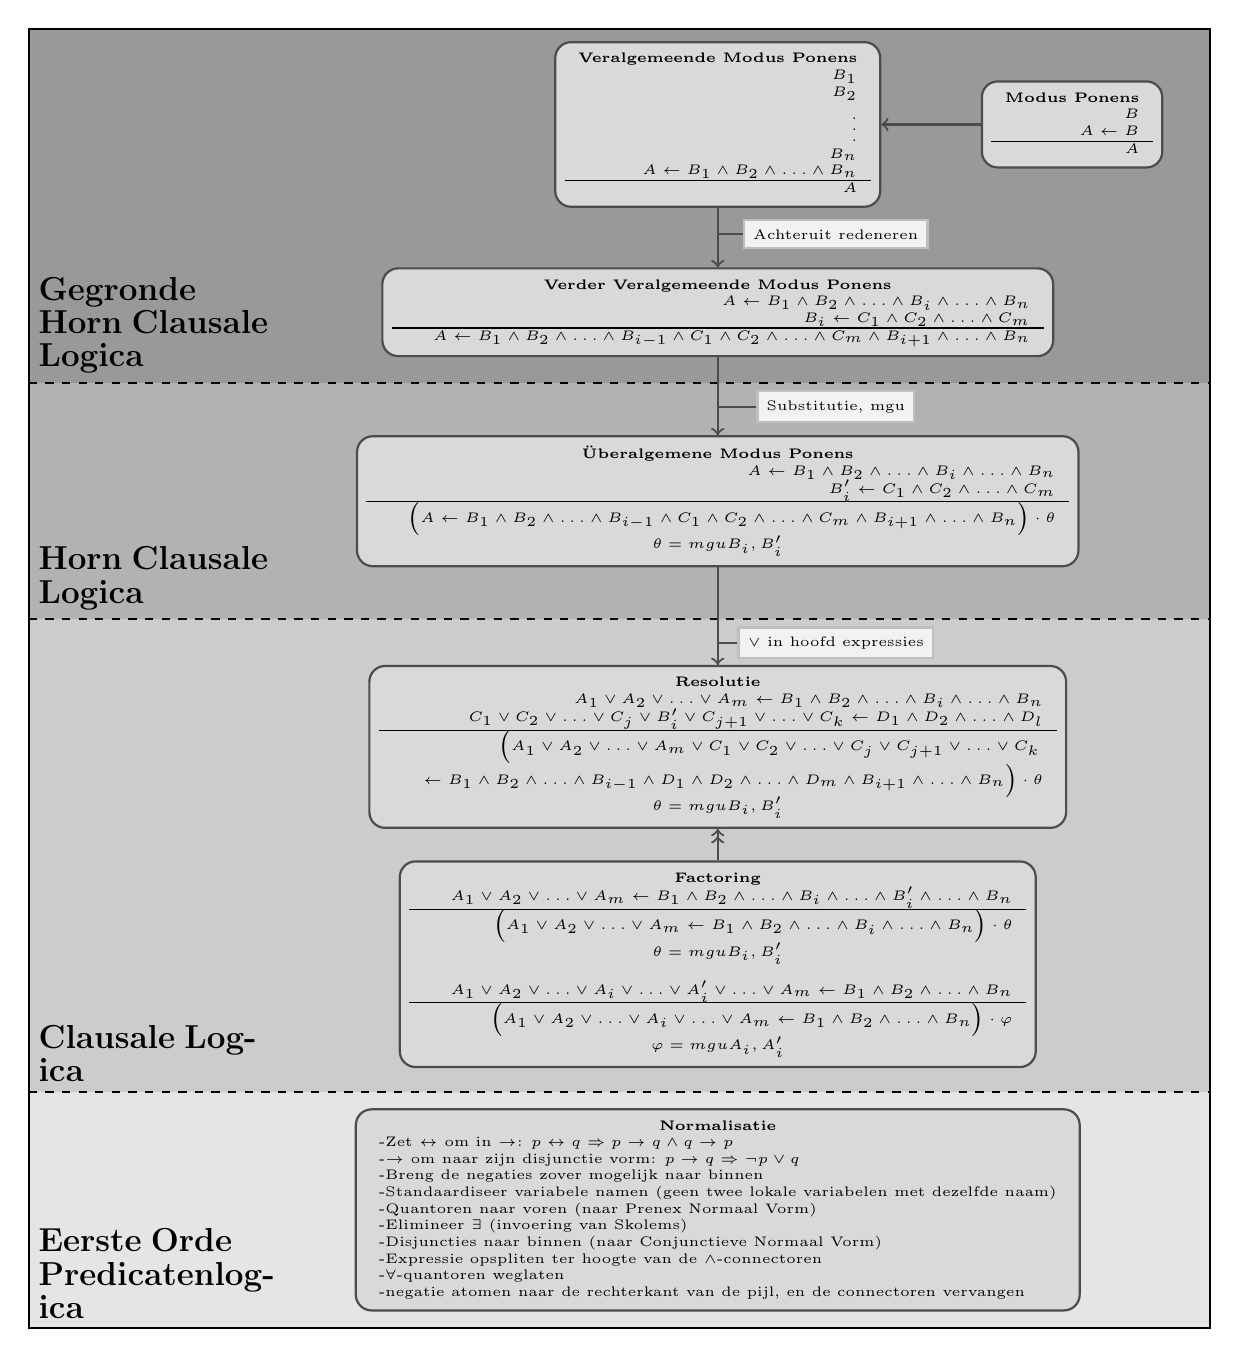
\begin{tikzpicture}[taal/.style={anchor=south west,text width=90pt},taalT/.style={draw=green,thick,fill=green!50},taalF/.style={draw=black!70,thick,fill=blue!50,rounded corners=2mm},concept/.style={draw=black!70,thick,fill=black!15,rounded corners=2mm},conceptgeneral/.style={thick,->,black!70},principle/.style={draw=black!25,thick,fill=black!5},principleused/.style={black!70,thick}]
\def\rectW{15};
\def\trapa{4.5};
\def\trapb{7.5};
\def\trapc{13.5};
\def\trapd{16.5};
\def\rectH{16.5};
\def\column{-0.5*\rectW+3.25};
\def\barW{\rectW-3.25};
\def\colF{4};
\def\xT{\column+2+0.3*\barW};
\def\xF{\column+2+0.5*\barW};
\def\xCa{\column+2+0.45*\barW};
\def\xCb{\column+2+0.55*\barW};
\def\xCc{\column+2+0.75*\barW};

\fill[black!40] (-0.5*\rectW,0) rectangle (0.5*\rectW,-\trapa);
\fill[black!30] (-0.5*\rectW,-\trapa) rectangle (0.5*\rectW,-\trapb);
\fill[black!20] (-0.5*\rectW,-\trapb) rectangle (0.5*\rectW,-\trapc);
\fill[black!10] (-0.5*\rectW,-\trapc) rectangle (0.5*\rectW,-\trapd);
\draw[thick] (-0.5*\rectW,0) rectangle (0.5*\rectW,-\rectH);
\draw[thick,dashed] (-0.5*\rectW,-\trapa) -- (0.5*\rectW,-\trapa);
\draw[thick,dashed] (-0.5*\rectW,-\trapb) -- (0.5*\rectW,-\trapb);
\draw[thick,dashed] (-0.5*\rectW,-\trapc) -- (0.5*\rectW,-\trapc);
%\draw[thick,dashed] (\column,0) -- (\column,-\rectH);

\node[taal] (trapaL) at (-0.5*\rectW,-\trapa) {\bf \large Gegronde Horn Clausale Logica};
\node[concept] (trapaC1) at (\xCc,-0.27*\trapa) {\tiny$\begin{array}{lr}\multicolumn{2}{c}{\mbox{\bf Modus Ponens}}\\&B\\\therefore&A\leftarrow B\\\hline&A\end{array}$};
\node[concept] (trapaC2) at (\xCa,-0.27*\trapa) {\tiny$\begin{array}{lr}\multicolumn{2}{c}{\mbox{\bf Veralgemeende Modus Ponens}}\\&B_1\\&B_2\\&\vdots\\&B_n\\\therefore&A\leftarrow B_1\wedge B_2\wedge\ldots\wedge B_n\\\hline&A\end{array}$};
\node[concept] (trapaC3) at (\xCa,-0.8*\trapa) {\tiny$\begin{array}{lr}\multicolumn{2}{c}{\mbox{\bf Verder Veralgemeende Modus Ponens}}\\&A\leftarrow B_1\wedge B_2\wedge\ldots\wedge B_i\wedge\ldots\wedge B_n\\\therefore&B_i\leftarrow C_1\wedge C_2\wedge\ldots\wedge C_m\\\hline&A\leftarrow B_1\wedge B_2\wedge\ldots\wedge B_{i-1}\wedge C_1\wedge C_2\wedge\ldots\wedge C_m\wedge B_{i+1}\wedge\ldots\wedge B_n\end{array}$};
\node[principle] (trapaP1) at (\xCb,-0.58*\trapa) {\tiny Achteruit redeneren};
\draw[principleused] (trapaC3.north) |- (trapaP1.west);
\draw[conceptgeneral] (trapaC1) -- (trapaC2);
\draw[conceptgeneral] (trapaC2) -- (trapaC3);

\node[taal] (trapbL) at (-0.5*\rectW,-\trapb) {\bf \large Horn Clausale Logica};
\node[concept] (trapbC1) at (\xCa,-0.5*\trapa-0.5*\trapb) {\tiny$\begin{array}{lr}\multicolumn{2}{c}{\mbox{\bf \"Uberalgemene Modus Ponens}}\\&A\leftarrow B_1\wedge B_2\wedge\ldots\wedge B_i\wedge\ldots\wedge B_n\\\therefore&B_i'\leftarrow C_1\wedge C_2\wedge\ldots\wedge C_m\\\hline&\left(A\leftarrow B_1\wedge B_2\wedge\ldots\wedge B_{i-1}\wedge C_1\wedge C_2\wedge\ldots\wedge C_m\wedge B_{i+1}\wedge\ldots\wedge B_n\right)\cdot\theta\\\multicolumn{2}{c}{\theta=\mathfunc{mgu}{B_i,B_i'}}\end{array}$};
\node[principle] (trapbP1) at (\xCb,-0.9*\trapa-0.1*\trapb) {\tiny Substitutie, mgu};
\draw[principleused] (trapbC1.north) |- (trapbP1.west);
\draw[conceptgeneral] (trapaC3) -- (trapbC1);

\node[taal] (trapcL) at (-0.5*\rectW,-\trapc) {\bf \large Clausale Logica};
\node[concept] (trapcC1) at (\xCa,-0.27*\trapc-0.73*\trapb) {\tiny$\begin{array}{lr}\multicolumn{2}{c}{\mbox{\bf Resolutie}}\\
&A_1\vee A_2\vee\ldots\vee A_m\leftarrow B_1\wedge B_2\wedge\ldots\wedge B_i\wedge\ldots\wedge B_n\\\therefore&C_1\vee C_2\vee\ldots\vee C_j\vee B_i'\vee C_{j+1}\vee\ldots\vee C_k\leftarrow D_1\wedge D_2\wedge\ldots\wedge D_l\\\hline&\left(A_1\vee A_2\vee\ldots\vee A_m\vee C_1\vee C_2\vee\ldots\vee C_j\vee C_{j+1}\vee\ldots\vee C_k\right.\\&\left.\leftarrow B_1\wedge B_2\wedge\ldots\wedge B_{i-1}\wedge D_1\wedge D_2\wedge\ldots\wedge D_m\wedge B_{i+1}\wedge\ldots\wedge B_n\right)\cdot\theta\\\multicolumn{2}{c}{\theta=\mathfunc{mgu}{B_i,B_i'}}\end{array}$};
\node[concept] (trapcC2) at (\xCa,-0.73*\trapc-0.27*\trapb) {\tiny$\begin{array}{lr}\multicolumn{2}{c}{\mbox{\bf Factoring}}\\\therefore&A_1\vee A_2\vee\ldots\vee A_m\leftarrow B_1\wedge B_2\wedge\ldots\wedge B_i\wedge\ldots\wedge B_i'\wedge\ldots\wedge B_n\\\hline&\left(A_1\vee A_2\vee\ldots\vee A_m\leftarrow B_1\wedge B_2\wedge\ldots\wedge B_i\wedge\ldots\wedge B_n\right)\cdot\theta\\\multicolumn{2}{c}{\theta=\mathfunc{mgu}{B_i,B_i'}}\\\\
\therefore&A_1\vee A_2\vee\ldots\vee A_i\vee\ldots\vee A_i'\vee\ldots\vee A_m\leftarrow B_1\wedge B_2\wedge\ldots\wedge B_n\\\hline&\left(A_1\vee A_2\vee\ldots\vee A_i\vee\ldots\vee A_m\leftarrow B_1\wedge B_2\wedge\ldots\wedge B_n\right)\cdot\varphi\\\multicolumn{2}{c}{\varphi=\mathfunc{mgu}{A_i,A_i'}}\end{array}$};
\node[principle] (trapcP1) at (\xCb,-0.95*\trapb-0.05*\trapc) {\tiny $\vee$ in hoofd expressies};
\draw[principleused] (trapcC1.north) |- (trapcP1.west);
\draw[conceptgeneral] (trapbC1) -- (trapcC1);
\draw[conceptgeneral,<<-] (trapcC1) -- (trapcC2);

\node[taal] (trapdL) at (-0.5*\rectW,-\trapd) {\bf \large Eerste Orde Predicatenlogica};
\node[concept] (trapaL) at (\xCa,-0.5*\trapd-0.5*\trapc) {\tiny$\begin{array}{l}\multicolumn{1}{c}{\mbox{\bf Normalisatie}}\\\mbox{-Zet $\leftrightarrow$ om in $\rightarrow$: $p\leftrightarrow q\Rightarrow p\rightarrow q\wedge q\rightarrow p$}\\\mbox{-$\rightarrow$ om naar zijn disjunctie vorm: $p\rightarrow q\Rightarrow \neg p\vee q$}\\\mbox{-Breng de negaties zover mogelijk naar binnen}\\\mbox{-Standaardiseer variabele namen (geen twee lokale variabelen met dezelfde naam)}\\\mbox{-Quantoren naar voren (naar Prenex Normaal Vorm)}\\\mbox{-Elimineer $\exists$ (invoering van Skolems)}\\\mbox{-Disjuncties naar binnen (naar Conjunctieve Normaal Vorm)}\\\mbox{-Expressie opspliten ter hoogte van de $\wedge$-connectoren}\\\mbox{-$\forall$-quantoren weglaten}\\\mbox{-negatie atomen naar de rechterkant van de pijl, en de connectoren vervangen}\end{array}$};
\end{tikzpicture}
\caption{Samenvattend schema van Automatisch Redeneren}
\end{figure}
\section{Metaheuristieken}
\begin{figure}[H]
\centering
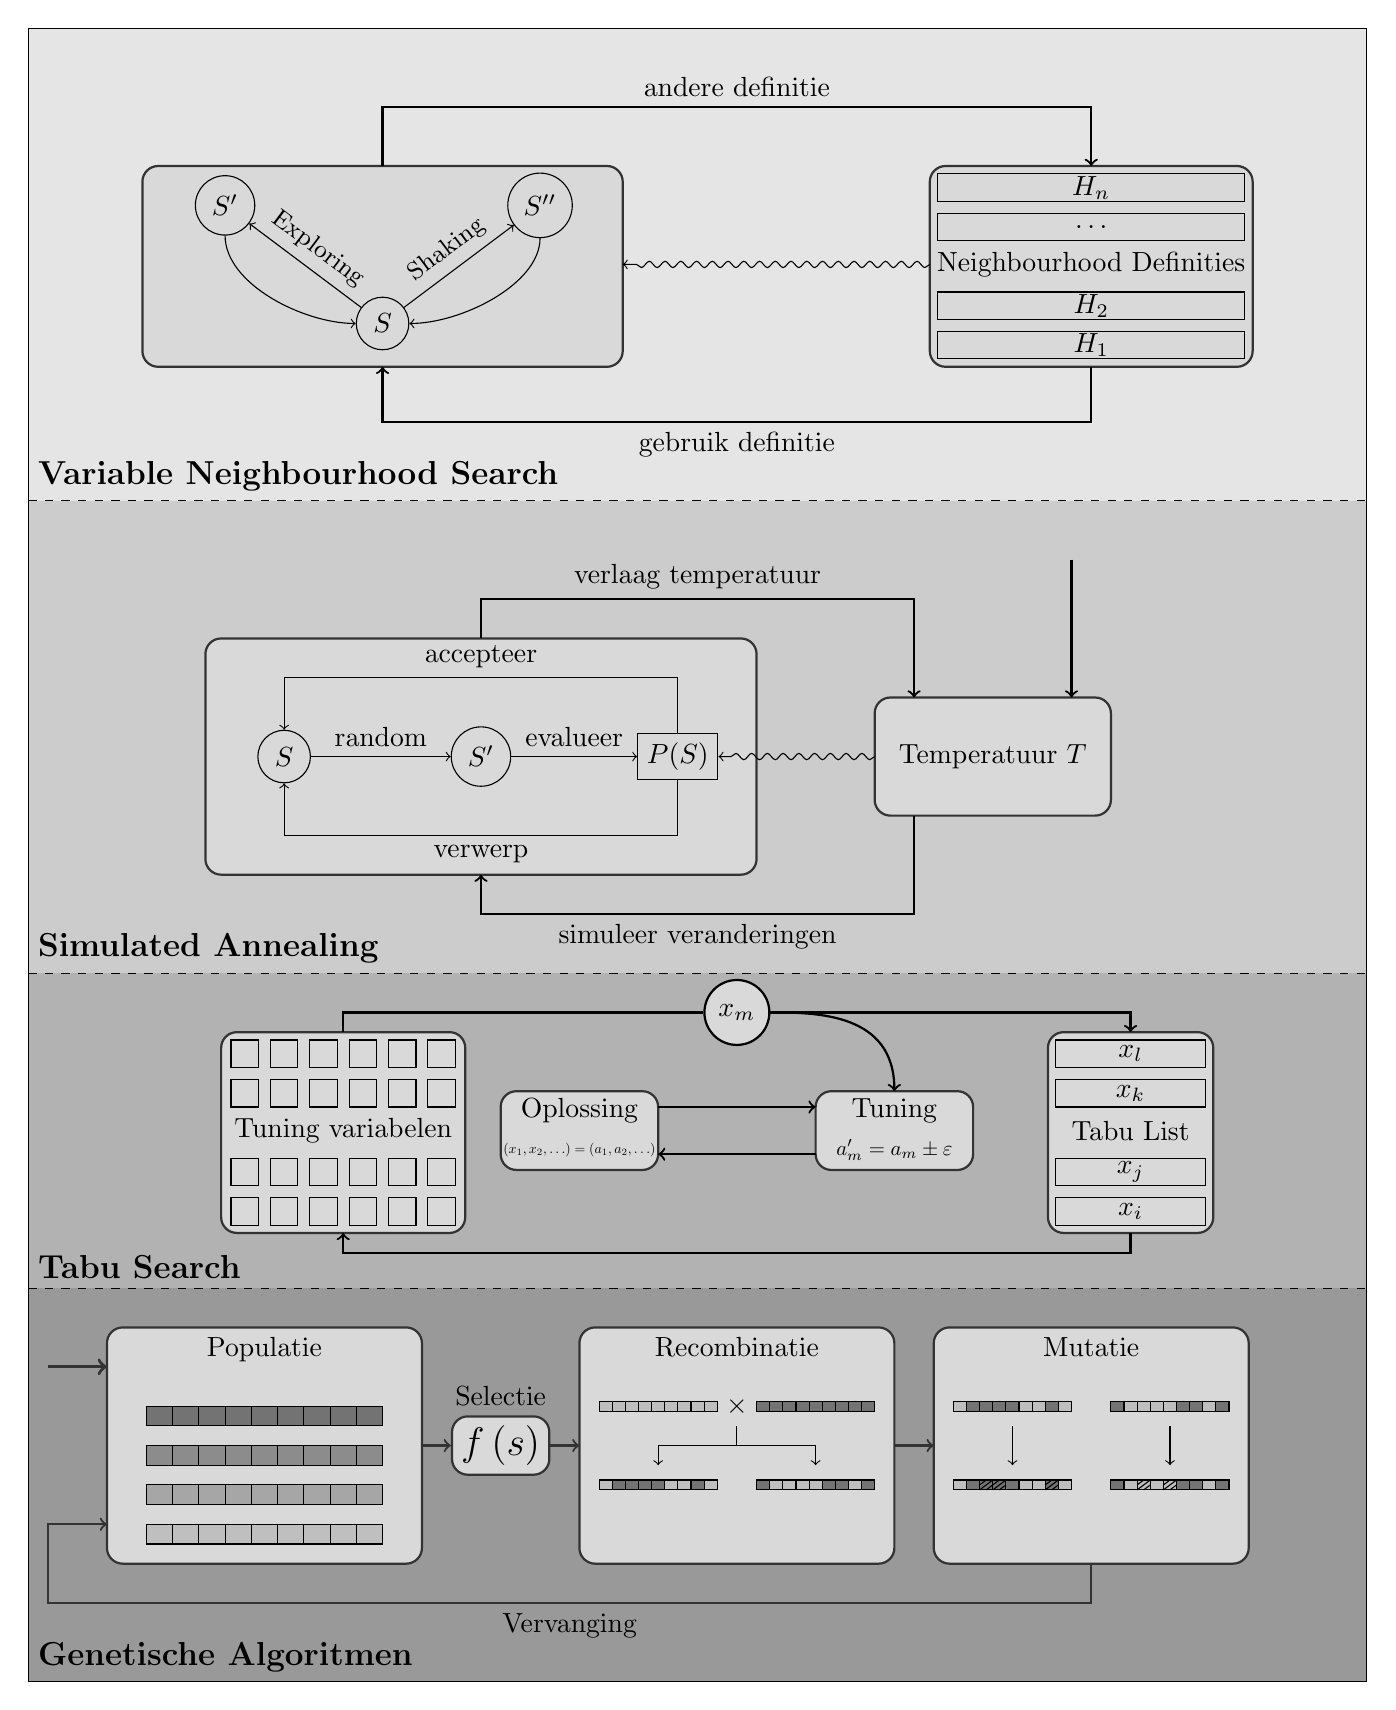
\begin{tikzpicture}[concclass/.style={anchor=south west},conceptgroup/.style={draw=black!80, thick,fill=black!15, rounded corners=2mm},conceptname/.style={anchor=north},cname/.style={conceptgroup},conceptarr/.style={black!80,thick,->}]
\fill[black!40] (-2,-0.5) rectangle (15,4.5);
\fill[black!30] (-2,4.5) rectangle (15,8.5);
\fill[black!20] (-2,8.5) rectangle (15,14.5);
\fill[black!10] (-2,14.5) rectangle (15,20.5);
\draw (-2,-0.5) rectangle (15,20.5);
\draw[dashed] (-2,4.5) -- (15,4.5);
\draw[dashed] (-2,8.5) -- (15,8.5);
\draw[dashed] (-2,14.5) -- (15,14.5);

\draw[concclass] (-2,-0.5) node{\bf \large Genetische Algoritmen};
\draw[conceptgroup] (-1,4) rectangle (3,1);
\node[conceptname] (Pop) at (1,4) {Populatie};
\foreach\y/\c in {1/25,2/35,3/45,4/55} {
  \fill[black!\c] (-0.5,0.5*\y+0.75) rectangle (2.5,0.5*\y+1);
  \draw[black] (-0.5,0.5*\y+0.75) rectangle (2.5,0.5*\y+1);
  \foreach \x in {1,2,...,8} {
    \draw[black] (-0.5+\x/3,0.5*\y+0.75) -- (-0.5+\x/3,0.5*\y+1);
  }
}
\draw[conceptarr,very thick] (-1.75,3.5) -- (-1,3.5);
\node[cname] (Eva) at (4,2.5) {\Large $f\left(s\right)$};
\node[conceptname,anchor=south] (Sel) at (Eva.north) {Selectie};
\draw[conceptarr] (3,2.5) -- (Eva);
\draw[conceptgroup] (5,4) rectangle (9,1);
\node[conceptname] (Pop) at (7,4) {Recombinatie};
\draw (7,3) node {$\times$};
\fill[black!25,draw=black] (5.25,2.9375) rectangle (6.75,3.0625);
\fill[black!55,draw=black] (7.25,2.9375) rectangle (8.75,3.0625);
\fill[black!25] (5.25,1.9375) rectangle (6.75,2.0625);
\fill[black!55] (7.25,1.9375) rectangle (8.75,2.0625);
\foreach \x/\y in {1/5,7/8} {
  \fill[black!55] (5.25+\x/6,1.9375) rectangle (5.25+\y/6,2.0625);
  \fill[black!25] (7.25+\x/6,1.9375) rectangle (7.25+\y/6,2.0625);
}
\draw (5.25,1.9375) rectangle (6.75,2.0625);
\draw (7.25,1.9375) rectangle (8.75,2.0625);
\draw (7,2.75) -- (7,2.5);
\draw[<->] (6,2.25) -- (6,2.5) -- (8,2.5) -- (8,2.25);
\foreach \x in {1,2,...,8} {
  \draw[black] (5.25+\x/6,2.9375) -- (5.25+\x/6,3.0625);
  \draw[black] (7.25+\x/6,2.9375) -- (7.25+\x/6,3.0625);
  \draw[black] (5.25+\x/6,1.9375) -- (5.25+\x/6,2.0625);
  \draw[black] (7.25+\x/6,1.9375) -- (7.25+\x/6,2.0625);
}
\draw[conceptarr] (Eva) -- (5,2.5);
\draw[conceptgroup] (9.5,4) rectangle (13.5,1);
\node[conceptname] (Pop) at (11.5,4) {Mutatie};
\fill[black!25] (9.75,2.9375) rectangle (11.25,3.0625);
\fill[black!55] (11.75,2.9375) rectangle (13.25,3.0625);
\fill[black!25] (9.75,1.9375) rectangle (11.25,2.0625);
\fill[black!55] (11.75,1.9375) rectangle (13.25,2.0625);
\foreach \x/\y in {1/5,7/8} {
  \fill[black!55] (9.75+\x/6,2.9375) rectangle (9.75+\y/6,3.0625);
  \fill[black!25] (11.75+\x/6,2.9375) rectangle (11.75+\y/6,3.0625);
  \fill[black!55] (9.75+\x/6,1.9375) rectangle (9.75+\y/6,2.0625);
  \fill[black!25] (11.75+\x/6,1.9375) rectangle (11.75+\y/6,2.0625);
}
\foreach \x in {2,3,7} {
  %\fill[gray] (9.75+\x/6,1.9375) rectangle (9.75+\x/6+1/6,2.0625);
  \draw (9.75+\x/6,1.9375) -- (9.75+\x/6+1/6,2.0625);
  \draw (9.75+1/12+\x/6,1.9375) -- (9.75+\x/6+1/6,2);
  \draw (9.75+\x/6,2) -- (9.75+\x/6+1/12,2.0625);
}
\foreach \x in {2,4} {
  %\fill[gray] (11.75+\x/6,1.9375) rectangle (11.75+\x/6+1/6,2.0625);
  \draw (11.75+\x/6,1.9375) -- (11.75+\x/6+1/6,2.0625);
  \draw (11.75+1/12+\x/6,1.9375) -- (11.75+\x/6+1/6,2);
  \draw (11.75+\x/6,2) -- (11.75+\x/6+1/12,2.0625);
}
\draw[->] (10.5,2.75) -- (10.5,2.25);
\draw[->] (12.5,2.75) -- (12.5,2.25);
\draw (9.75,2.9375) rectangle (11.25,3.0625);
\draw (11.75,2.9375) rectangle (13.25,3.0625);
\draw (9.75,1.9375) rectangle (11.25,2.0625);
\draw (11.75,1.9375) rectangle (13.25,2.0625);
\foreach \x in {1,2,...,8} {
  \draw[black] (9.75+\x/6,2.9375) -- (9.75+\x/6,3.0625);
  \draw[black] (11.75+\x/6,2.9375) -- (11.75+\x/6,3.0625);
  \draw[black] (9.75+\x/6,1.9375) -- (9.75+\x/6,2.0625);
  \draw[black] (11.75+\x/6,1.9375) -- (11.75+\x/6,2.0625);
}
\draw[conceptarr] (9,2.5) -- (9.5,2.5);
\draw[conceptarr] (11.5,1) -- (11.5,0.5) to node[black,midway,below]{Vervanging} (-1.75,0.5) -- (-1.75,1.5) -- (-1,1.5);

\draw[concclass] (-2,4.5) node{\bf \large Tabu Search};
\draw[concclass] (-2,8.5) node{\bf \large Simulated Annealing};
\draw[concclass] (-2,14.5) node{\bf \large Variable Neighbourhood Search};
%\draw (0,9) node{\bf \large Optimal Search};
\begin{scope}[xshift=12 cm,yshift=6.5 cm]
\draw[conceptgroup] (-1.05,-1.3) rectangle (1.05,1.25);
\draw (0,0) node {Tabu List};
\foreach\y/\t in {1/i,2/j,4/k,5/l} {
  \draw (-0.95,-1.7+0.5*\y) rectangle (0.95,-1.35+0.5*\y);
  \draw (0,-1.525+0.5*\y) node{$x_\t$};
}
\draw[conceptgroup] (-11.55,-1.3) rectangle (-8.45,1.25);
\draw (-10,0) node {Tuning variabelen};
\foreach\y in {1,2,4,5} {
  \foreach\x in {0,1,2,3,4,5} {
    \draw (-11.425+0.5*\x,-1.7+0.5*\y) rectangle ++(0.35,0.35);
  }
}
\draw[conceptgroup] (-8,-0.5) rectangle (-6,0.5);
\draw (-7,0.25) node {Oplossing};
\draw (-7,-0.25) node[scale=0.5] {$\left(x_1,x_2,\ldots\right)=\left(a_1,a_2,\ldots\right)$};
\draw[conceptgroup] (-4,-0.5) rectangle (-2,0.5);
\draw (-3,-0.25) node[scale=0.75] {$a_m'=a_m\pm\varepsilon$};
\draw (-3,0.25) node {Tuning};
\node[conceptgroup,draw=black,circle,thick] (V) at (-5,1.5) {$x_m$};
\draw[thick,->] (-10,1.25) |- (V) -| (0,1.25);
\draw[thick,->] (0,-1.3) |- (-5,-1.55) -| (-10,-1.3);
\draw[thick,->] (-6,0.3) -- (-4,0.3);
\draw[thick,->] (-4,-0.3) -- (-6,-0.3);
\draw[thick,->] (V) .. controls ++(1,0) and (-3,1.5) .. (-3,0.5);
\end{scope}
\begin{scope}[xshift=3.75 cm,yshift=11.25 cm]
\draw[conceptgroup] (5,-0.75) rectangle (8,0.75);
\draw (6.5,0) node {Temperatuur $T$};
\draw[conceptgroup] (-3.5,-1.5) rectangle (3.5,1.5);
\node[draw=black,circle] (S1) at (-2.5,0) {$S$};
\node[draw=black,circle] (S2) at (0,0) {$S'$};
\node[draw=black,rectangle] (P) at (2.5,0) {$P(S)$};
\draw[->] (S1) to node[midway,sloped,above]{random} (S2);
\draw[->] (S2) to node[midway,sloped,above]{evalueer} (P);
\draw[->] (P.south) -- (2.5,-1) to node[below,midway,sloped] {verwerp} (-2.5,-1) -- (S1);
\draw[->] (P.north) -- (2.5,1) to node[above,midway,sloped] {accepteer} (-2.5,1) -- (S1);
\draw[->,decorate,decoration={snake,amplitude=.4mm,segment length=2mm,post length=1mm}] (5,0) -- (P);
\draw[thick,->] (7.5,2.5) -- (7.5,0.75);
\draw[thick,->] (0,1.5) -- (0,2) to node[midway,sloped,above]{verlaag temperatuur} (5.5,2) -- (5.5,0.75);
\draw[thick,->] (5.5,-0.75) -- (5.5,-2) to node[midway,sloped,below]{simuleer veranderingen} (0,-2) -- (0,-1.5);
\end{scope}
\begin{scope}[xshift=11.5 cm,yshift=17.5 cm]
\draw[conceptgroup] (-2.05,-1.3) rectangle (2.05,1.25);
\draw (0,0) node {Neighbourhood Definities};
\foreach\y/\t in {1/\mathfrak{H}_1,2/\mathfrak{H}_2,4/\ldots,5/\mathfrak{H}_n} {
  \draw (-1.95,-1.7+0.5*\y) rectangle (1.95,-1.35+0.5*\y);
  \draw (0,-1.525+0.5*\y) node{$\t$};
}
\draw[conceptgroup] (-12.05,-1.3) rectangle (-5.95,1.25);
\node[draw=black,circle] (S) at (-9,-0.75) {$S$};
\node[draw=black,circle] (S1) at (-11,0.75) {$S'$};
\node[draw=black,circle] (S2) at (-7,0.75) {$S''$};
\draw[->] (S) to node[sloped,midway,above]{\small{Exploring}} (S1);
\draw[->] (S) to node[sloped,midway,above]{\small{Shaking}} (S2);
\draw[->] (S1) .. controls ++(0,-1) and (-10,-0.75) .. (S);
\draw[->] (S2) .. controls ++(0,-1) and (-8,-0.75) .. (S);
\draw[->,decorate,decoration={snake,amplitude=.4mm,segment length=2mm,post length=1mm}] (-2.05,0) -- (-5.95,0);
\draw[->,thick] (0,-1.3) -- (0,-2) to node[midway,sloped,below]{gebruik definitie} (-9,-2) -- (-9,-1.3);
\draw[->,thick] (-9,1.25) -- (-9,2) to node[midway,sloped,above]{andere definitie} (0,2) -- (0,1.25);
\end{scope}
\end{tikzpicture}
\caption{Samenvattend schema van Metaheuristieken}
\end{figure}

%\section{Afbeeldingen bij Concept Learning}
%\begin{figure}[H]
%\centering
%\begin{tikzpicture}[activeGeneral/.style={draw=green,thick,fill=green!50,shape=circle},passivGeneral/.style={draw=green!50,thick,fill=green!20,shape=circle},activeSpecial/.style={draw=red,thick,fill=red!50,shape=circle},passivSpecial/.style={draw=red!50,thick,fill=red!20,shape=circle},fitgs/.style={->,dashed}]
%\def\dx{0.4};
%\def\dy{-.75};
%\def\dr{0.2};
%\coordinate (f1Offset) at (-18*\dx,-8*\dy);
%\coordinate (f2Offset) at (-6*\dx,-8*\dy);
%\coordinate (f3Offset) at (6*\dx,-8*\dy);
%\coordinate (f4Offset) at (-18*\dx,0);
%\coordinate (f5Offset) at (-6*\dx,0);
%\coordinate (f6Offset) at (6*\dx,0);

%\draw[very thick](-18*\dx,0) -- (18*\dx,0);
%\draw[very thick](-6*\dx,-8*\dy) -- (-6*\dx,8*\dy);
%\draw[very thick](6*\dx,-8*\dy) -- (6*\dx,8*\dy);
%\draw[very thick] (-18*\dx,-8*\dy) rectangle (18*\dx,8*\dy);

%\draw (f1Offset) node[anchor=north west]{Initial state};
%\node[activeGeneral] (f1TopG) at (-12*\dx,-7*\dy) { };
%\node[activeSpecial] (f1TopS) at (-12*\dx,-\dy) { };
%\draw (f1TopG.south) node[anchor=north]{$G=\left\{\left[\mbox{?},\mbox{?},\ldots,\mbox{?}\right]\right\}$};
%\draw (f1TopS.north) node[anchor=south]{$S=\left\{\perp\right\}$};

%\draw (f2Offset) node[anchor=north west]{Negative test-situation};
%\node[passivGeneral] (f2TopG) at (0,-7*\dy) { };
%\node[activeGeneral] (f2L1G1) at (-2*\dx,-6*\dy) { };
%\node[activeGeneral] (f2L1G2) at (0,-6*\dy) { };
%\node[activeGeneral] (f2L1G3) at (2*\dx,-6*\dy) { };
%\node[activeSpecial] (f2TopS) at (0,-\dy) { };
%\draw(f2TopG) -- (f2L1G1);
%\draw(f2TopG) -- (f2L1G2);
%\draw(f2TopG) -- (f2L1G3);
%\draw (f2L1G2.south) node[anchor=north]{$G=\left\{h_1,h_2,h_3\right\}$};
%\draw (f2TopS.north) node[anchor=south]{$S=\left\{\perp\right\}$};

%\draw (f3Offset) node[anchor=north west]{Positive test-situation};
%\node[passivGeneral] (f3TopG) at (12*\dx,-7*\dy) { };
%\node[activeGeneral] (f3L1G1) at (10*\dx,-6*\dy) { };
%\node[activeGeneral] (f3L1G2) at (12*\dx,-6*\dy) { };
%\node[activeGeneral] (f3L1G3) at (14*\dx,-6*\dy) { };
%\node[passivSpecial] (f3TopS) at (12*\dx,-\dy) { };
%\node[activeSpecial] (f3L1S1) at (12*\dx,-2*\dy) { };
%\draw(f3TopG) -- (f3L1G1);
%\draw(f3TopG) -- (f3L1G2);
%\draw(f3TopG) -- (f3L1G3);
%\draw(f3TopS) -- (f3L1S1);
%\draw (f3L1G2.south) node[anchor=north]{$G=\left\{h_1,h_2,h_3\right\}$};
%\draw (f3L1S1.north) node[anchor=south]{$S=\left\{h_1'\right\}$};

%\draw (f4Offset) node[anchor=north west]{Negative test-situation};
%\node[passivGeneral] (f4TopG) at (-12*\dx,\dy) { };
%\node[passivGeneral] (f4L1G1) at (-14*\dx,2*\dy) { };
%\node[activeGeneral] (f4L2G11) at (-15*\dx,3*\dy) { };
%\node[activeGeneral] (f4L2G12) at (-13*\dx,3*\dy) { };
%\node[activeGeneral] (f4L1G2) at (-12*\dx,2*\dy) { };
%\node[passivGeneral] (f4L1G3) at (-10*\dx,2*\dy) { };
%\node[activeGeneral] (f4L2G31) at (-10*\dx,3*\dy) { };
%\node[passivSpecial] (f4TopS) at (-12*\dx,7*\dy) { };
%\node[activeSpecial] (f4L1S1) at (-12*\dx,6*\dy) { };
%\coordinate (f4Gmiddle) at (-12*\dx,3*\dy-\dr);
%\draw(f4TopG) -- (f4L1G1);
%\draw(f4L1G1) -- (f4L2G11);
%\draw(f4L1G1) -- (f4L2G12);
%\draw(f4TopG) -- (f4L1G2);
%\draw(f4TopG) -- (f4L1G3);
%\draw(f4L1G3) -- (f4L2G31);
%\draw(f4TopS) -- (f4L1S1);
%\draw[fitgs] (f4L2G11) -- (f4L1S1);
%\draw[fitgs] (f4L2G31) -- (f4L1S1);
%\draw (f4Gmiddle.south) node[anchor=north]{$G=\left\{h_{1\,1},h_2,h_{3\,1}\right\}$};
%\draw (f4L1S1.north) node[anchor=south]{$S=\left\{h_1'\right\}$};
%\draw ($(f4L2G21) - (\dr,\dr)$) -- ($(f4L2G21) + (\dr,\dr)$);
%\draw ($(f4L2G21) - (\dr,-\dr)$) -- ($(f4L2G21) + (\dr,-\dr)$);
%\end{tikzpicture}
%\caption{Version spaces in actie}
%\end{figure}
% \section{Afbeeldingen bij Constraint Processing}
% \begin{figure}[H]
% \centering
% \begin{tikzpicture}[rotate=90,val/.style={rotate=90}]
% \def\dxa{4};
% \def\dxb{1};
% \def\dxc{1};
% \def\dxd{0.75};
% \def\xlabel{-1.5*\dxa-1.5*\dxb-1.5*\dxc-1.5};
% \def\la{-1};
% \def\lb{-3};
% \def\lbCa{-3.5};
% \def\lc{-5};
% \def\lcCa{-5.5};
% \def\lcCb{-6};
% \def\ld{-7};
% \def\ldCa{-7.5};
% \def\ldCb{-8};
% \def\ldCc{-8.5};
% \coordinate (root) at (0,0);
% 
% \draw (\xlabel,\la) node[val,anchor=west]{$z_1$};
% \draw (\xlabel,\lb) node[val,anchor=west]{$z_2$};
% \draw (\xlabel,\lbCa) node[val,anchor=west]{$c\left(z_1,z_2\right)$};
% \draw (\xlabel,\lc) node[val,anchor=west]{$z_3$};
% \draw (\xlabel,\lcCa) node[val,anchor=west]{$c\left(z_1,z_3\right)$};
% \draw (\xlabel,\lcCb) node[val,anchor=west]{$c\left(z_2,z_3\right)$};
% \draw (\xlabel,\ld) node[val,anchor=west]{$z_4$};
% \draw (\xlabel,\ldCa) node[val,anchor=west]{$c\left(z_1,z_4\right)$};
% \draw (\xlabel,\ldCb) node[val,anchor=west]{$c\left(z_2,z_4\right)$};
% \draw (\xlabel,\ldCc) node[val,anchor=west]{$c\left(z_3,z_4\right)$};
% 
% \node[val] (l1a) at (-1.5*\dxa,\la) {$a_{1\,1}$};
% \node[val] (l1b) at (-0.5*\dxa,\la) {$a_{1\,2}$};
% \node[val] (l1c) at (0.5*\dxa,\la) {$\ldots$};
% \node[val] (l1d) at (1.5*\dxa,\la) {$a_{1\,n_1}$};
% \draw (root) -- (l1a) (root) -- (l1b) (root) -- (l1c) (root) -- (l1d);
% 
% \node[val] (l2aa) at (-1.5*\dxa-1.5*\dxb,\lb) {$a_{2\,1}$};
% \node[val] (l2ab) at (-1.5*\dxa-0.5*\dxb,\lb) {$a_{2\,2}$};
% \node[val] (l2ac) at (-1.5*\dxa+0.5*\dxb,\lb) {$\ldots$};
% \node[val] (l2ad) at (-1.5*\dxa+1.5*\dxb,\lb) {$a_{2\,n_2}$};
% \node[val] (l2aaC1) at (-1.5*\dxa-1.5*\dxb,\lbCa) {$\XBox$};
% \node[val] (l2abC1) at (-1.5*\dxa-0.5*\dxb,\lbCa) {$\CheckedBox$};
% \node[val] (l2acC1) at (-1.5*\dxa+0.5*\dxb,\lbCa) {$\ldots$};
% \node[val] (l2adC1) at (-1.5*\dxa+1.5*\dxb,\lbCa) {$\XBox$};
% \draw (l1a) -- (l2aa) (l1a) -- (l2ab) (l1a) -- (l2ac) (l1a) -- (l2ad);
% 
% \node[val] (l2ba) at (-0.5*\dxa-1.5*\dxb,\lb) {$a_{2\,1}$};
% \node[val] (l2bb) at (-0.5*\dxa-0.5*\dxb,\lb) {$a_{2\,2}$};
% \node[val] (l2bc) at (-0.5*\dxa+0.5*\dxb,\lb) {$\ldots$};
% \node[val] (l2bd) at (-0.5*\dxa+1.5*\dxb,\lb) {$a_{2\,n_2}$};
% \node[val] (l2baC1) at (-0.5*\dxa-1.5*\dxb,\lbCa) {$\XBox$};
% \node[val] (l2bbC1) at (-0.5*\dxa-0.5*\dxb,\lbCa) {$\XBox$};
% \node[val] (l2bcC1) at (-0.5*\dxa+0.5*\dxb,\lbCa) {$\ldots$};
% \node[val] (l2bdC1) at (-0.5*\dxa+1.5*\dxb,\lbCa) {$\CheckedBox$};
% \draw (l1b) -- (l2ba) (l1b) -- (l2bb) (l1b) -- (l2bc) (l1b) -- (l2bd);
% 
% \node[val] (l2da) at (1.5*\dxa-1.5*\dxb,\lb) {$a_{2\,1}$};
% \node[val] (l2db) at (1.5*\dxa-0.5*\dxb,\lb) {$a_{2\,2}$};
% \node[val] (l2dc) at (1.5*\dxa+0.5*\dxb,\lb) {$\ldots$};
% \node[val] (l2dd) at (1.5*\dxa+1.5*\dxb,\lb) {$a_{2\,n_2}$};
% \node[val] (l2daC1) at (1.5*\dxa-1.5*\dxb,\lbCa) {$\CheckedBox$};
% \node[val] (l2dbC1) at (1.5*\dxa-0.5*\dxb,\lbCa) {$\XBox$};
% \node[val] (l2dcC1) at (1.5*\dxa+0.5*\dxb,\lbCa) {$\ldots$};
% \node[val] (l2ddC1) at (1.5*\dxa+1.5*\dxb,\lbCa) {$\XBox$};
% \draw (l1d) -- (l2da) (l1d) -- (l2db) (l1d) -- (l2dc) (l1d) -- (l2dd);
% 
% \node[val] (l3aba) at (-1.5*\dxa-0.5*\dxb-1.5*\dxc,\lc) {$a_{3\,1}$};
% \node[val] (l3abb) at (-1.5*\dxa-0.5*\dxb-0.5*\dxc,\lc) {$a_{3\,2}$};
% \node[val] (l3abc) at (-1.5*\dxa-0.5*\dxb+0.5*\dxc,\lc) {$\ldots$};
% \node[val] (l3abd) at (-1.5*\dxa-0.5*\dxb+1.5*\dxc,\lc) {$a_{3\,n_3}$};
% \node[val] (l3abaC1) at (-1.5*\dxa-0.5*\dxb-1.5*\dxc,\lcCa) {$\CheckedBox$};
% \node[val] (l3abbC1) at (-1.5*\dxa-0.5*\dxb-0.5*\dxc,\lcCa) {$\CheckedBox$};
% \node[val] (l3abcC1) at (-1.5*\dxa-0.5*\dxb+0.5*\dxc,\lcCa) {$\ldots$};
% \node[val] (l3abdC1) at (-1.5*\dxa-0.5*\dxb+1.5*\dxc,\lcCa) {$\CheckedBox$};
% \node[val] (l3abaC2) at (-1.5*\dxa-0.5*\dxb-1.5*\dxc,\lcCb) {$\XBox$};
% \node[val] (l3abbC2) at (-1.5*\dxa-0.5*\dxb-0.5*\dxc,\lcCb) {$\CheckedBox$};
% \node[val] (l3abcC2) at (-1.5*\dxa-0.5*\dxb+0.5*\dxc,\lcCb) {$\ldots$};
% \node[val] (l3abdC2) at (-1.5*\dxa-0.5*\dxb+1.5*\dxc,\lcCb) {$\XBox$};
% \draw (l2abC1) -- (l3aba) (l2abC1) -- (l3abb) (l2abC1) -- (l3abc) (l2abC1) -- (l3abd);
% 
% \node[val] (l3bda) at (-0.5*\dxa+1.5*\dxb-1.5*\dxc,\lc) {$a_{3\,1}$};
% \node[val] (l3bdb) at (-0.5*\dxa+1.5*\dxb-0.5*\dxc,\lc) {$a_{3\,2}$};
% \node[val] (l3bdc) at (-0.5*\dxa+1.5*\dxb+0.5*\dxc,\lc) {$\ldots$};
% \node[val] (l3bdd) at (-0.5*\dxa+1.5*\dxb+1.5*\dxc,\lc) {$a_{3\,n_3}$};
% \node[val] (l3bdaC1) at (-0.5*\dxa+1.5*\dxb-1.5*\dxc,\lcCa) {$\CheckedBox$};
% \node[val] (l3bdbC1) at (-0.5*\dxa+1.5*\dxb-0.5*\dxc,\lcCa) {$\CheckedBox$};
% \node[val] (l3bdcC1) at (-0.5*\dxa+1.5*\dxb+0.5*\dxc,\lcCa) {$\ldots$};
% \node[val] (l3bddC1) at (-0.5*\dxa+1.5*\dxb+1.5*\dxc,\lcCa) {$\CheckedBox$};
% \node[val] (l3bdaC2) at (-0.5*\dxa+1.5*\dxb-1.5*\dxc,\lcCb) {$\CheckedBox$};
% \node[val] (l3bdbC2) at (-0.5*\dxa+1.5*\dxb-0.5*\dxc,\lcCb) {$\XBox$};
% \node[val] (l3bdcC2) at (-0.5*\dxa+1.5*\dxb+0.5*\dxc,\lcCb) {$\ldots$};
% \node[val] (l3bddC2) at (-0.5*\dxa+1.5*\dxb+1.5*\dxc,\lcCb) {$\CheckedBox$};
% \draw (l2bdC1) -- (l3bda) (l2bdC1) -- (l3bdb) (l2bdC1) -- (l3bdc) (l2bdC1) -- (l3bdd);
% 
% \node[val] (l3daa) at (1.5*\dxa-1.5*\dxb-1.5*\dxc,\lc) {$a_{3\,1}$};
% \node[val] (l3dab) at (1.5*\dxa-1.5*\dxb-0.5*\dxc,\lc) {$a_{3\,2}$};
% \node[val] (l3dac) at (1.5*\dxa-1.5*\dxb+0.5*\dxc,\lc) {$\ldots$};
% \node[val] (l3dad) at (1.5*\dxa-1.5*\dxb+1.5*\dxc,\lc) {$a_{3\,n_3}$};
% \node[val] (l3daaC1) at (1.5*\dxa-1.5*\dxb-1.5*\dxc,\lcCa) {$\CheckedBox$};
% \node[val] (l3dabC1) at (1.5*\dxa-1.5*\dxb-0.5*\dxc,\lcCa) {$\XBox$};
% \node[val] (l3dacC1) at (1.5*\dxa-1.5*\dxb+0.5*\dxc,\lcCa) {$\ldots$};
% \node[val] (l3dadC1) at (1.5*\dxa-1.5*\dxb+1.5*\dxc,\lcCa) {$\XBox$};
% \node[val] (l3daaC2) at (1.5*\dxa-1.5*\dxb-1.5*\dxc,\lcCb) {$\XBox$};
% \node[val] (l3dabC2) at (1.5*\dxa-1.5*\dxb-0.5*\dxc,\lcCb) {$\ $};
% \node[val] (l3dacC2) at (1.5*\dxa-1.5*\dxb+0.5*\dxc,\lcCb) {$\ldots$};
% \node[val] (l3dadC2) at (1.5*\dxa-1.5*\dxb+1.5*\dxc,\lcCb) {$ $};
% \draw (l2daC1) -- (l3daa) (l2daC1) -- (l3dab) (l2daC1) -- (l3dac) (l2daC1) -- (l3dad);
% 
% \node[val,blue] (l4abba) at (-1.5*\dxa-0.5*\dxb-0.5*\dxc-1.5*\dxd,\ld) {$a_{4\,1}$};
% \node[val,blue] (l4abbb) at (-1.5*\dxa-0.5*\dxb-0.5*\dxc-0.5*\dxd,\ld) {$a_{4\,2}$};
% \node[val,blue] (l4abbc) at (-1.5*\dxa-0.5*\dxb-0.5*\dxc+0.5*\dxd,\ld) {$\ldots$};
% \node[val,blue] (l4abbd) at (-1.5*\dxa-0.5*\dxb-0.5*\dxc+1.5*\dxd,\ld) {$a_{4\,n_4}$};
% \node[val,blue] (l4abbaC1) at (-1.5*\dxa-0.5*\dxb-0.5*\dxc-1.5*\dxd,\ldCa) {$\XBox$};
% \node[val,blue] (l4abbbC1) at (-1.5*\dxa-0.5*\dxb-0.5*\dxc-0.5*\dxd,\ldCa) {$\CheckedBox$};
% \node[val,blue] (l4abbcC1) at (-1.5*\dxa-0.5*\dxb-0.5*\dxc+0.5*\dxd,\ldCa) {$\ldots$};
% \node[val,blue] (l4abbdC1) at (-1.5*\dxa-0.5*\dxb-0.5*\dxc+1.5*\dxd,\ldCa) {$\XBox$};
% \node[val,blue] (l4abbaC2) at (-1.5*\dxa-0.5*\dxb-0.5*\dxc-1.5*\dxd,\ldCb) {$ $};
% \node[val,blue] (l4abbbC2) at (-1.5*\dxa-0.5*\dxb-0.5*\dxc-0.5*\dxd,\ldCb) {$\XBox$};
% \node[val,blue] (l4abbcC2) at (-1.5*\dxa-0.5*\dxb-0.5*\dxc+0.5*\dxd,\ldCb) {$\XBox$};
% \node[val,blue] (l4abbdC2) at (-1.5*\dxa-0.5*\dxb-0.5*\dxc+1.5*\dxd,\ldCb) {$ $};
% \node[val,blue] (l4abbaC3) at (-1.5*\dxa-0.5*\dxb-0.5*\dxc-1.5*\dxd,\ldCc) {$ $};
% \node[val,blue] (l4abbbC3) at (-1.5*\dxa-0.5*\dxb-0.5*\dxc-0.5*\dxd,\ldCc) {$ $};
% \node[val,blue] (l4abbcC3) at (-1.5*\dxa-0.5*\dxb-0.5*\dxc+0.5*\dxd,\ldCc) {$ $};
% \node[val,blue] (l4abbdC3) at (-1.5*\dxa-0.5*\dxb-0.5*\dxc+1.5*\dxd,\ldCc) {$ $};
% \draw (l3abbC2) -- (l4abba) (l3abbC2) -- (l4abbb) (l3abbC2) -- (l4abbc) (l3abbC2) -- (l4abbd);
% 
% \node[val] (l4bdaa) at (-0.5*\dxa+1.5*\dxb-1.5*\dxc-1.5*\dxd,\ld) {$a_{4\,1}$};
% \node[val] (l4bdab) at (-0.5*\dxa+1.5*\dxb-1.5*\dxc-0.5*\dxd,\ld) {$a_{4\,2}$};
% \node[val] (l4bdac) at (-0.5*\dxa+1.5*\dxb-1.5*\dxc+0.5*\dxd,\ld) {$\ldots$};
% \node[val] (l4bdad) at (-0.5*\dxa+1.5*\dxb-1.5*\dxc+1.5*\dxd,\ld) {$a_{4\,n_4}$};
% \node[val,green] (l4bdaaC1) at (-0.5*\dxa+1.5*\dxb-1.5*\dxc-1.5*\dxd,\ldCa) {$\CheckedBox$};
% \node[val,green] (l4bdabC1) at (-0.5*\dxa+1.5*\dxb-1.5*\dxc-0.5*\dxd,\ldCa) {$\CheckedBox$};
% \node[val,green] (l4bdacC1) at (-0.5*\dxa+1.5*\dxb-1.5*\dxc+0.5*\dxd,\ldCa) {$\ldots$};
% \node[val,green] (l4bdadC1) at (-0.5*\dxa+1.5*\dxb-1.5*\dxc+1.5*\dxd,\ldCa) {$\XBox$};
% \node[val,green] (l4bdaaC2) at (-0.5*\dxa+1.5*\dxb-1.5*\dxc-1.5*\dxd,\ldCb) {$\CheckedBox$};
% \node[val,green] (l4bdabC2) at (-0.5*\dxa+1.5*\dxb-1.5*\dxc-0.5*\dxd,\ldCb) {$\CheckedBox$};
% \node[val,green] (l4bdacC2) at (-0.5*\dxa+1.5*\dxb-1.5*\dxc+0.5*\dxd,\ldCb) {$\ldots$};
% \node[val,green] (l4bdadC2) at (-0.5*\dxa+1.5*\dxb-1.5*\dxc+1.5*\dxd,\ldCb) {$ $};
% \node[val] (l4bdaaC3) at (-0.5*\dxa+1.5*\dxb-1.5*\dxc-1.5*\dxd,\ldCc) {$\XBox$};
% \node[val] (l4bdabC3) at (-0.5*\dxa+1.5*\dxb-1.5*\dxc-0.5*\dxd,\ldCc) {$\XBox$};
% \node[val] (l4bdacC3) at (-0.5*\dxa+1.5*\dxb-1.5*\dxc+0.5*\dxd,\ldCc) {$\ldots$};
% \node[val] (l4bdadC3) at (-0.5*\dxa+1.5*\dxb-1.5*\dxc+1.5*\dxd,\ldCc) {$ $};
% \draw (l3bdaC2) -- (l4bdaa) (l3bdaC2) -- (l4bdab) (l3bdaC2) -- (l4bdac) (l3bdaC2) -- (l4bdad);
% 
% \node[val] (l4bdda) at (-0.5*\dxa+1.5*\dxb+1.5*\dxc-1.5*\dxd,\ld) {$a_{4\,1}$};
% \node[val] (l4bddb) at (-0.5*\dxa+1.5*\dxb+1.5*\dxc-0.5*\dxd,\ld) {$a_{4\,2}$};
% \node[val] (l4bddc) at (-0.5*\dxa+1.5*\dxb+1.5*\dxc+0.5*\dxd,\ld) {$\ldots$};
% \node[val] (l4bddd) at (-0.5*\dxa+1.5*\dxb+1.5*\dxc+1.5*\dxd,\ld) {$a_{4\,n_4}$};
% \node[val,green] (l4bddaC1) at (-0.5*\dxa+1.5*\dxb+1.5*\dxc-1.5*\dxd,\ldCa) {$\CheckedBox$};
% \node[val,green] (l4bddbC1) at (-0.5*\dxa+1.5*\dxb+1.5*\dxc-0.5*\dxd,\ldCa) {$\CheckedBox$};
% \node[val,green] (l4bddcC1) at (-0.5*\dxa+1.5*\dxb+1.5*\dxc+0.5*\dxd,\ldCa) {$\ldots$};
% \node[val,green] (l4bdddC1) at (-0.5*\dxa+1.5*\dxb+1.5*\dxc+1.5*\dxd,\ldCa) {$\XBox$};
% \node[val,green] (l4bddaC2) at (-0.5*\dxa+1.5*\dxb+1.5*\dxc-1.5*\dxd,\ldCb) {$\CheckedBox$};
% \node[val,green] (l4bddbC2) at (-0.5*\dxa+1.5*\dxb+1.5*\dxc-0.5*\dxd,\ldCb) {$\CheckedBox$};
% \node[val,green] (l4bddcC2) at (-0.5*\dxa+1.5*\dxb+1.5*\dxc+0.5*\dxd,\ldCb) {$\ldots$};
% \node[val,green] (l4bdddC2) at (-0.5*\dxa+1.5*\dxb+1.5*\dxc+1.5*\dxd,\ldCb) {$ $};
% \node[val] (l4bddaC3) at (-0.5*\dxa+1.5*\dxb+1.5*\dxc-1.5*\dxd,\ldCc) {$\XBox$};
% \node[val] (l4bddbC3) at (-0.5*\dxa+1.5*\dxb+1.5*\dxc-0.5*\dxd,\ldCc) {$\CheckedBox$};
% \node[val] (l4bddcC3) at (-0.5*\dxa+1.5*\dxb+1.5*\dxc+0.5*\dxd,\ldCc) {$\ldots$};
% \node[val] (l4bdddC3) at (-0.5*\dxa+1.5*\dxb+1.5*\dxc+1.5*\dxd,\ldCc) {$ $};
% \draw (l3bddC2) -- (l4bdda) (l3bddC2) -- (l4bddb) (l3bddC2) -- (l4bddc) (l3bddC2) -- (l4bddd);
% 
% %backtracking algorithms
% %chronological backtracking
% \draw[rounded corners,red,->] (root) -- (l1a.north) -- (l2aa.north) -- (l2ab.north) -- (l3aba.north) -- (l3abb.north) -- (l4abba.north) -- (l4abbb.north) -- (l4abbc.north) -- (l4abbd.north) -- (l3abc.north) -- (l3abd.north) -- (l2ac.north) -- (l2ad.north) -- (l1b.north) -- (l2ba.north) -- (l2bb.north) -- (l2bc.north) -- (l2bd.north) -- (l3bda.north) -- (l4bdaa.north) -- (l4bdab.north) -- (l4bdac.north) -- (l4bdad.north) -- (l3bdb.north) -- (l3bdc.north) -- (l3bdd.north) -- (l4bdda.north) -- (l4bddb.north) -- (l4bddc.north) -- (l4bddd.north) -- (l1c.north) -- (l1d.north) -- (l2da.north) -- (l3daa.north) -- (l3dab.north) -- (l3dac.north) -- (l3dad.north) -- (l2db.north) -- (l2dc.north) -- (l2dd.north);
% %backjumping
% \draw[rounded corners,blue,->] (root) -- (l1a.south) -- (l2aa.south) -- (l2ab.south) -- (l3aba.south) -- (l3abb.south) -- (l4abba.south) -- (l4abbb.south) -- (l4abbc.south) -- (l4abbd.south) -- (l2ac.south) -- (l2ad.south) -- (l1b.south) -- (l2ba.south) -- (l2bb.south) -- (l2bc.south) -- (l2bd.south) -- (l3bda.south) -- (l4bdaa.south) -- (l4bdab.south) -- (l4bdac.south) -- (l4bdad.south) -- (l3bdb.south) -- (l3bdc.south) -- (l3bdd.south) -- (l4bdda.south) -- (l4bddb.south) -- (l4bddc.south) -- (l4bddd.south) -- (l1c.south) -- (l1d.south) -- (l2da.south) -- (l3daa.south) -- (l3dab.south) -- (l3dac.south) -- (l3dad.south) -- (l2db.south) -- (l2dc.south) -- (l2dd.south);
% \end{tikzpicture}
% \caption{Voorstelling van een OR-tree met diepte $4$}%. Hierbij is een oplossing $z_1=a_{1\,2}$, $z_2=a_{2\,n_2}$, $z_3=a_{3\,n_3}$ en $z_4=a_{4\,2}$
% \label{fig:orTree}
% \end{figure}
% \begin{figure}[H]
% \centering
% \begin{tikzpicture}[var/.style={draw=black,shape=circle},rule/.style={fill=red!50,draw=red!80},ra/.style={red},rar/.style={ra,->}]
% \def\dx{4};
% \def\dy{3};
% \def\r{0.125};
% \node[var] (z1) at (0,\dy) {$z_1$};
% \node[var] (z2) at (-\dx,0) {$z_2$};
% \node[var] (z3) at (0,-\dy) {$z_3$};
% \node[var] (z4) at (\dx,0) {$z_4$};
% \node[rule] (r1) at (\dx,\dy) {$\forall i:\neg c\left(z_1=a_{1\,i},z_4=a_{4\,2}\right)$};
% 
% \node (d1) at (z1.north) [anchor=south]{$\left\{a_{1\,1},a_{1\,2},\ldots,a_{1\,n_1}\right\}$};
% \node (d2) at (z2.west) [anchor=east]{$\left\{a_{2\,1},a_{2\,2},\ldots,a_{2\,n_2}\right\}$};
% \node (d3) at (z3.south) [anchor=north]{$\left\{a_{3\,1},a_{3\,2},\ldots,a_{3\,n_3}\right\}$};
% \node (d4) at (z4.east) [anchor=west]{$\left\{a_{4\,1},a_{4\,2},\ldots,a_{4\,n_4}\right\}$};
% \node (d4c) at (d4.south west) [anchor=north west,red]{$\left\{a_{4\,1},\ldots,a_{4\,n_4}\right\}$};
% 
% \draw (z1) to node[above,midway,sloped]{$c\left(z_1,z_2\right)$} (z2) to node[sloped,above,midway]{$c\left(z_2,z_3\right)$} (z3) to node[above,sloped,midway]{$c\left(z_3,z_4\right)$} (z4) to node[above,sloped,midway]{$c\left(z_1,z_4\right)$} (z1);
% \draw (z1) to node[above,near start,sloped]{$c\left(z_1,z_3\right)$} (z3);
% \draw (z2) to node[above,midway,sloped]{$c\left(z_2,z_4\right)$} (-\r,0) arc(180:0:\r) -- (z4);
% \draw[rar] (z1) -- (r1);
% \draw[rar] (z4) -- (r1);
% \draw[rar] (r1) -- (d4);
% \draw[ra] (d4.north west) -- (d4.south east);
% \draw[ra] (d4.south west) -- (d4.north east);
% \end{tikzpicture}
% \caption{Beginstaat van een Constraint Netwerk, met een relaxatie in het rood}
% \label{fig:constraintNetwork}
% \end{figure}

%\newpage
%\section{Afbeeldingen bij Automatisch Redeneren}
%\begin{figure}[H]
%\centering
%\begin{tikzpicture}
%\def\dx{60pt};
%\def\dy{30pt};
%\draw (0,0) ellipse (140pt and 70pt);
%\draw (-60pt,-20pt) ellipse (60pt and 35pt) node{Atomaire Proposities};
%\draw (0pt,30pt) ellipse (40pt and 20pt) node{Connectieven};
%\draw (60pt,-20pt) ellipse (45pt and 20pt) node{Punctuaties};
%\end{tikzpicture}
%\caption{Alfabet van Propositielogica}
%\end{figure}